\chapter{Time-Resolved Emittance Measurements}

Emittance is used as one of the main metrics to determine the quality of a charged particle beam.
Beam emittance determines the `focusability' of a beam which determines the size of the probe for electron and ion microscopes and is equivalent to the coherence of for synchrotrons, \glspl{xfel} and diffraction experiments.

Time-resolved measurements of emittance provide a powerful diagnostic for improvement of charged particle beams.
Elucidation of temporal emittance behaviour has the potential to permit better understanding of the processes involved in the creation and propagation of charged particle beam and thus could be a useful tool in improving these devices.
Time-resolved emittance has been performed previously using a pulsed \gls{mcp}~\cite{yoshida_simple_2001} and with optical transition radiation~\cite{le_sage_time-resolved_2002}.
This chapter presents a simple and novel method of measuring time-resolved emittance that is applicable to a wide range of charged particle sources and has the potential to be performed with a single-shot measurement.

The emittance of a \gls{caeis} is important to all of it's potential applications and the time-resolution provided by the technique described in this chapter will be a useful tool to examine the behaviour of the source and hopefully provide avenues for improvement.

Time resolved emittance measurements are useful {\color{red} (for what? check references for specific applications)} and have been achieved in a number of ways.
One method is to use a gated systems where the detector is only turned on for a short interval and the interval is adjusted from shot-to-shot to build up a temporal profile of the emittance measurement~\cite{bekefi_temporal_1987,yoshida_simple_2001}.
Another method is \gls{otr} which examines the radiation from a thin foil in order to determine the spatial profile and divergence of the particle beam and thus the emittance which has been time-resolved using a streak camera~\cite{fiorito_optical_1994}.
{\color{red}I don't really know how OTR works yet so I should read more or just not mention it.}

The method examined here for time-resolved emittance measurement is an adaption of the pepperpot methed that achieves the time resolution through streaking.
Streaking of charged particle beams involves applying a changing electric field to the beam in order to move it across the detector.
The streaking technique has been used previously for a number of measurements and is central to the operation of streak cameras.
Streaking has been used to provide time-resolution to ultrafast diffraction experiments using an rf deflecting cavity to $\sim$\unit[200][fs] resolution\cite{li_note:_2010}.
Streaked diffraction experiments have the potential to reveal dynamic information and due to the potential for single-shot measurements could be a useful tool on the road towards the `molecular movie'.

This chapter examines time-resolved emittance measurements through the streaking of pepperpots; including the theory involved, various technical considerations, example measurements and implementation of this technique with the \gls{caeis} at the University of Melbourne.


\section{Emittance}

A given ensemble of particles can be described by its density in six-dimensional phase space, $(x, p_x, y, p_x, z, p_z)$ where $(x, y, z)$ are the positions and $(p_x, p_y, p_z)$ are the momenta of each particle.
The extent of the beam in phase space is called the \emph{emittance}, $\epsilon$, of the beam.
Each cartesian direction is examined separately, $(\epsilon_x, x, p_x)$, $(\epsilon_y, y, p_y)$ and $(\epsilon_z, z, p_z)$ where $z$ is the optic axis of the beam.

Typically the gradients of trajectories in $x$-$z$ and $y$-$z$ are measured rather than the momenta.
These gradients are referred to as the divergence and are defined as $x^\prime \equiv \frac{dx}{dz} = \frac{v_x}{v_z}$.
The space of $(x, x^\prime)$ is referred to as trace-space.
An example of the trace-space occupied by a beam is shown in Figure~\ref{figure:emittance_example}.
The \emph{emittance} can be defined as
\begin{equation}
\epsilon^x \equiv \frac{A^x}{\pi}
\end{equation}
where $A^x$ is the area occupied by the beam in trace space.

\begin{figure}
\center
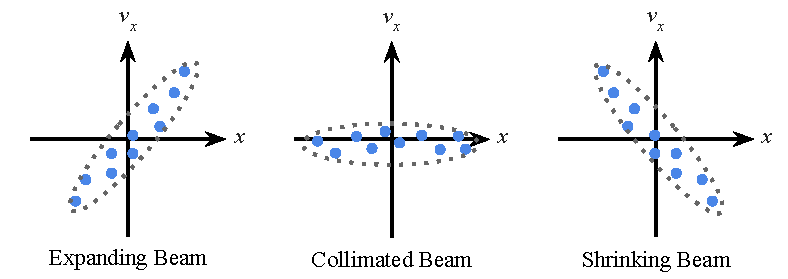
\includegraphics{part2/Figs/EmittanceExample.pdf}
\caption{An example of the trace-space occupied by an expanding, collimated and shrinking beam. The dotted line indicates the area occupied by the beam, the emittance.}
\label{figure:emittance_example}
\end{figure}

The density, $\rho$, of a beam of $N$ particles in trace space can usually be described by a Gaussian:
\begin{equation}\label{trace_space_density}
\rho(x, x^\prime) = N exp\left[ \frac{-(\sigma_{22}x^2-2\sigma_{12}xx^\prime+\sigma_{11}x^{\prime2}}{2|\sigma|} \right]
\end{equation}
where $|\sigma|$ is the determinant of the symmetric beam matrix,
\begin{equation}
\sigma = \begin{pmatrix} \sigma_{11} & \sigma_{12} \\ \sigma_{21} & \sigma_{22} \end{pmatrix}.
\end{equation}
$\sigma_{11}$ is the standard deviation of $x$, $\sigma_{22}$ the standard deviation of $x^\prime$ and $\sigma_{12}=\sigma_{21}$ indicates the coupling between $x$ and $x^\prime$. The \emph{emittance} can also be defined as
\begin{equation}\label{eq:emittancewithdeterminant}
\epsilon^x \equiv \sqrt{|\sigma|} = \sqrt{\sigma_{11}\sigma_{22}-\sigma_{12}^2}
\end{equation}

The \emph{\gls{rms} emittance} is a more practical measure and is defined as
\begin{equation}\label{emittance}
\epsilon \equiv \sqrt{\langle x^2\rangle \langle x^{\prime 2}\rangle - \langle x x^\prime\rangle^2}.
\end{equation}

\section{Measurement}

Directly calculating the emittance of an ensemble with Equation~\ref{emittance} requires full knowledge of the position and momenta of the particles which is difficult as beam monitors tend to only measure the transverse positions of particles.
There are a number of methods to practically calculate the emittance of a particle beam, namely pepperpots, the multiple profile method methods and the quadrupole method.

\subsection{Pepperpots}

The pepperpot method uses a beam mask, consisting of an array of small holes, to obscure the beam which is then propagated and detected downstream.
by examining the size of the spots on the detector the divergence of the beam can be estimated and thus the emittance of the beam can be calculated.
Ideally the extent of the array should be larger than the size of the beam and the holes are as small as is practicle while maintaining sufficient flux and ensuring the spots on the detector do not overlap.
The name refers to the similarity of the simplest beam mask to the perforated lid of a container for pepper.

A useful derivation of this technique is presented in Ref.~\cite{zhang_emittance_1996} with the one dimensional result:

\begin{dmath}\label{equation:pepperpot}
\epsilon_x^2 = \left\langle x^2\right\rangle \left\langle x^{\prime2}\right\rangle - \left\langle xx^\prime\right\rangle^2\allowbreak
\approx \frac{1}{N^2} \left\{\left[\sum_{j=1}^p{n_j\left(x_{sj}-\bar{x}\right)^2}\right] \left[ \sum_{j=1}^p{\left[n_j\sigma_{x_j^\prime}^2 + n_j\left(\bar{x_j^\prime}-\bar{x^\prime}\right)^2\right]}\right] - \left[ \sum_{j=1}^p{n_jx_{sj}\bar{x_j^\prime}-N\bar{x}\bar{x^\prime}}\right]^2\right\}
\end{dmath}
where;
\begin{itemize}
\item $N$ is the total number of particles after the beam mask,
\item $p$ is the total number of holes in the $x$ direction,
\item $n_j$ is the number of particles passing through the $j$-th hole and hitting the detector,
\item $x_{sj}$ is position of the $j$-th hole,
\item $\bar{x}$ is the mean position of the holes,
\item $\sigma_{x_j^\prime}$ is the \gls{rms} divergence of the $j$-th beamlet,
\item $\bar{x_j^\prime}$ is the mean divergence of the $j$-th beamlet, and
\item $\bar{x^\prime}$ is the mean divergence of all beamlets.
\end{itemize}

An example pepperpot mask and detected beamlets are shown in Figure~\ref{figure:pepperpot_example}.
This equation can be implemented by appropriately rotating the detected beamlets and then performing row and column sums of the pixels followed by application of Equation~\ref{equation:pepperpot} for $x$ and $y$.

\begin{figure}
\center
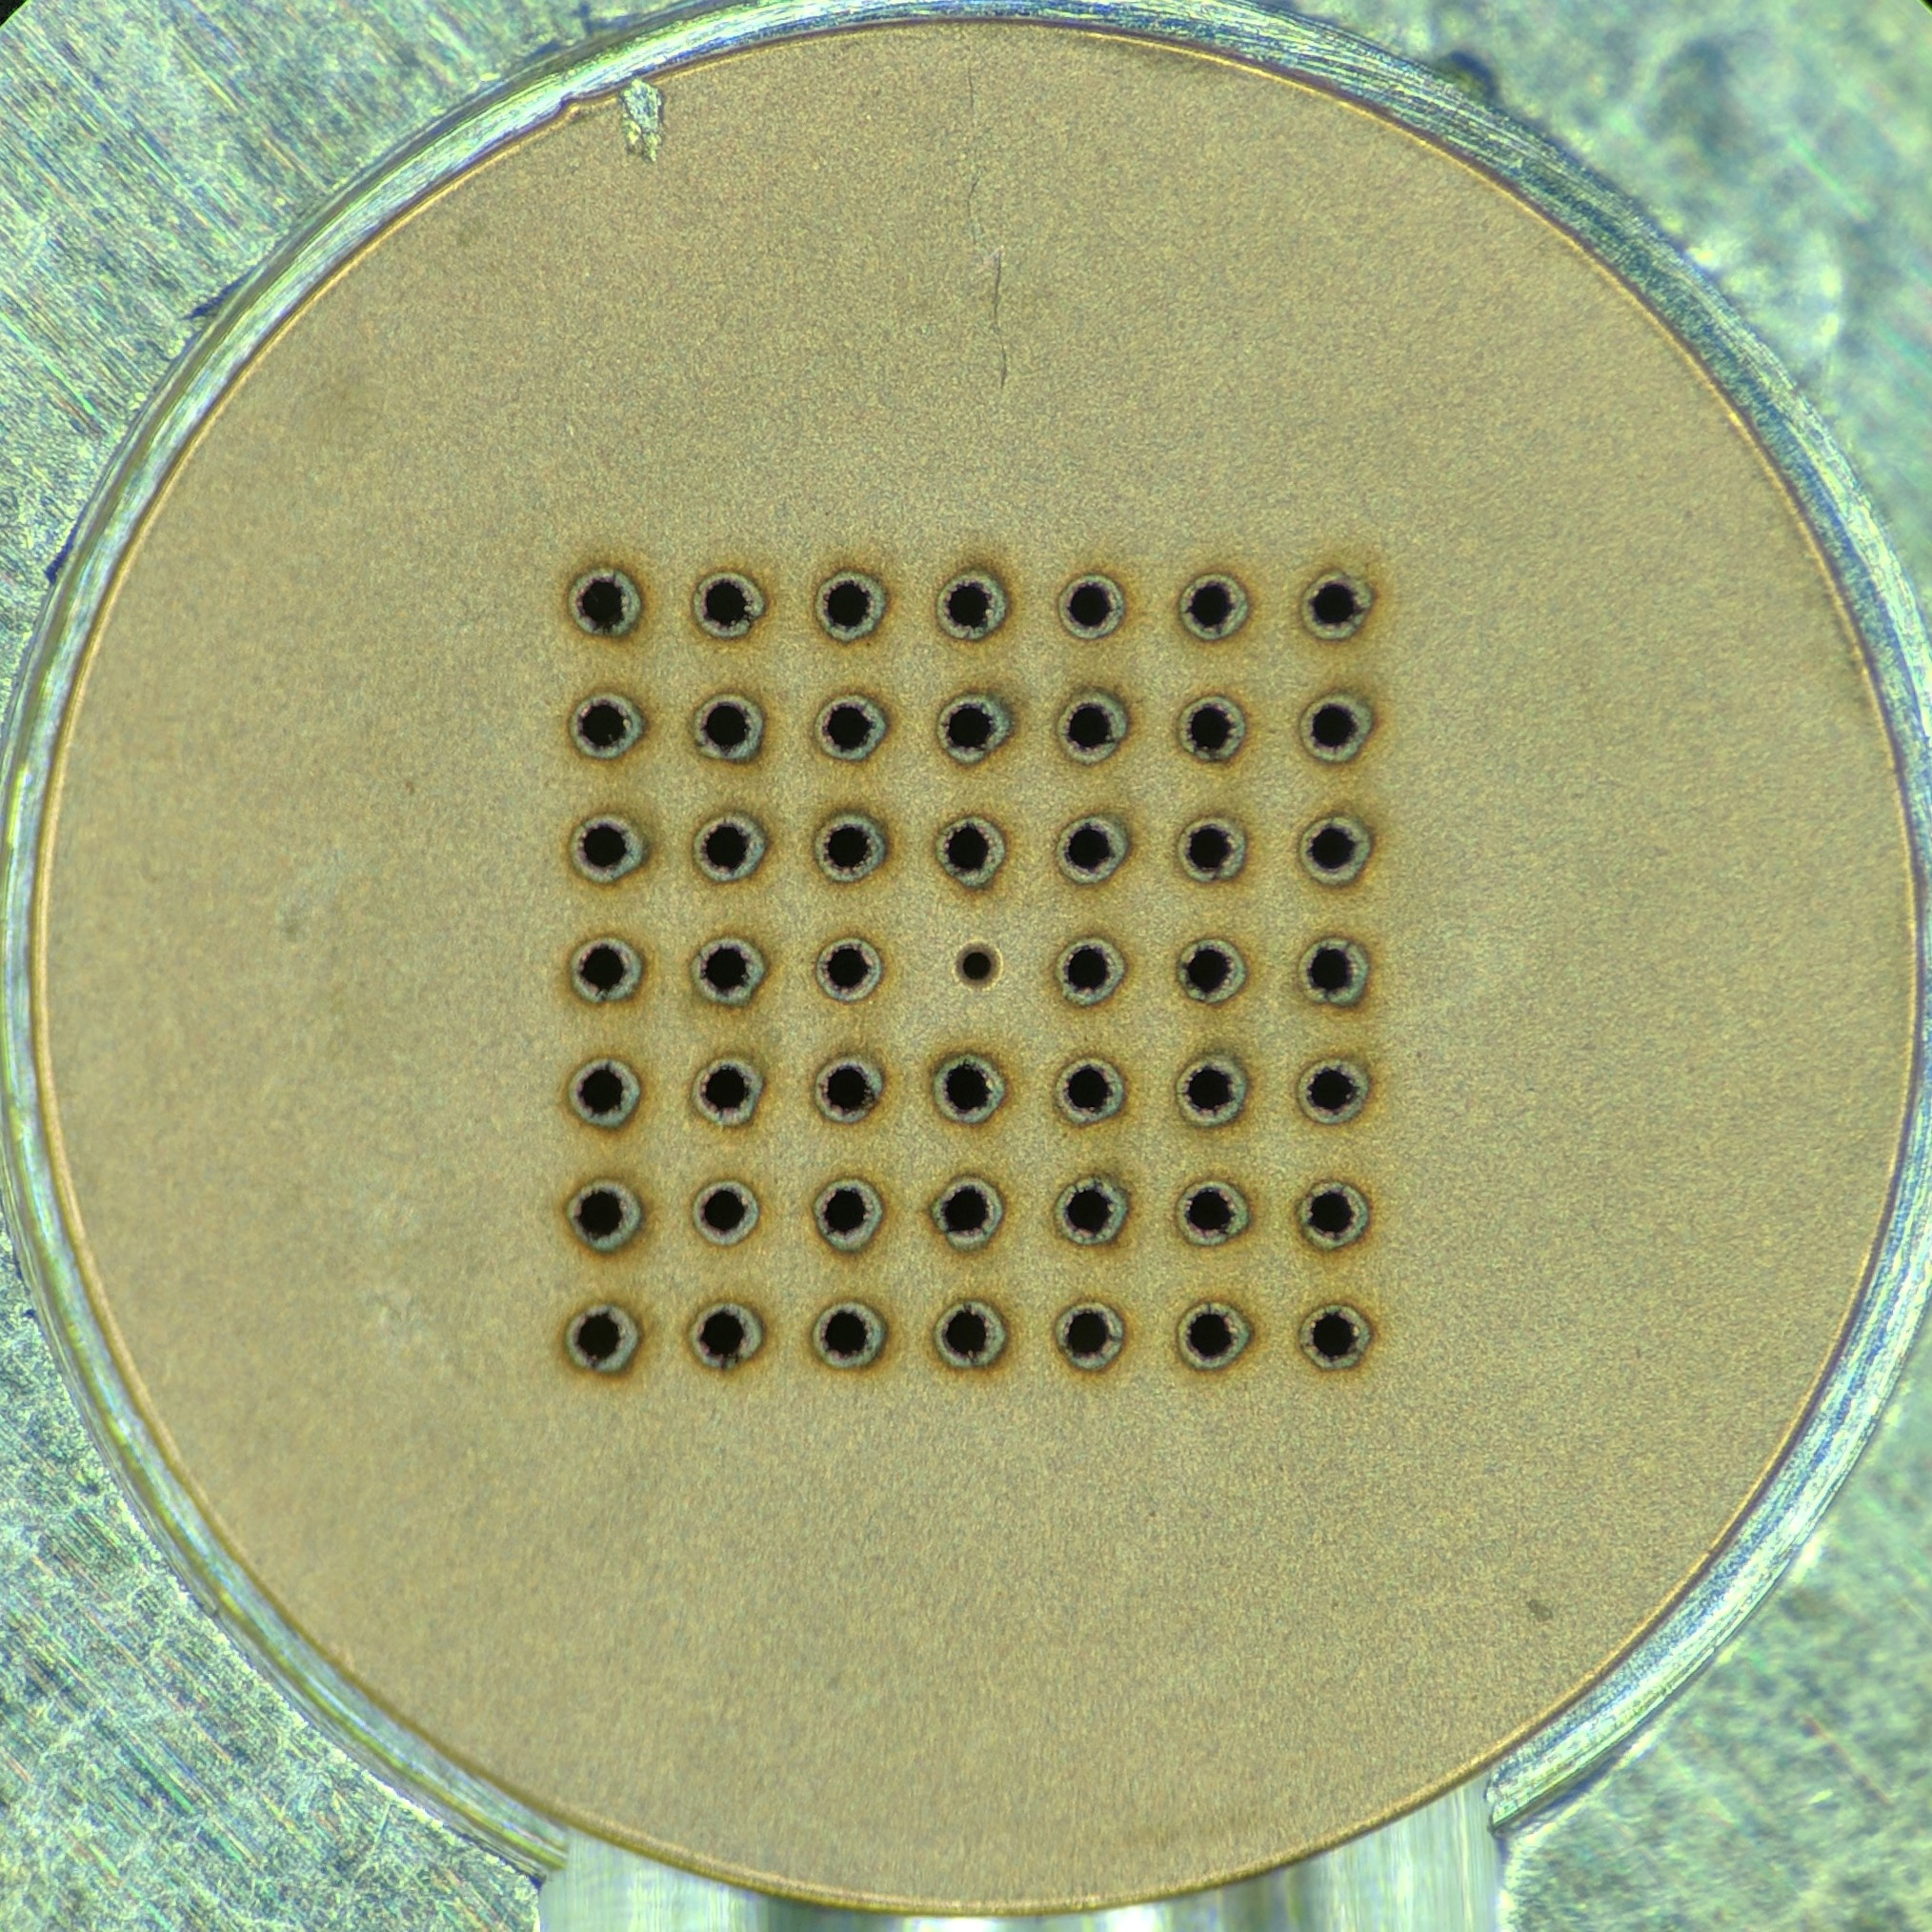
\includegraphics[width=0.49\linewidth]{part2/Figs/example_pepperpot_mask.jpg}
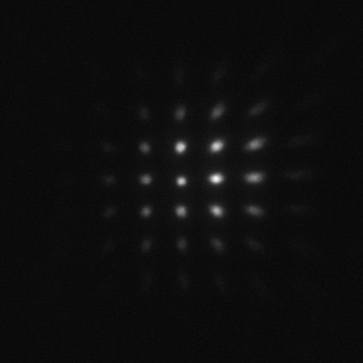
\includegraphics[width=0.49\linewidth]{part2/Figs/example_pepperpot_detector_linear.png}
\caption{An example a pepperpot mask (left) and a corresponding set of beamlets on the detector.}
\label{figure:pepperpot_example}
\end{figure}

\subsubsection{Time Resolution with Streaking}
1d pepperpots, streaked across the detector

\subsection{Multi-profile Method}

If a beam can be described by $\sigma^0$ at $z_0$ and by $\sigma^1$ at $z_1$ then the transformation matrix, $\mathbf{R}_{12}$ from $z_0$ to $z_1$ is
\begin{equation}
\mathbf{R} = \begin{pmatrix} R_{11} & R_{12} \\ R_{21} & R_{22} \end{pmatrix}
\end{equation}
and
\begin{equation}
\sigma^1 = \mathbf{R}\sigma^0\mathbf{R}^T
\end{equation}
where $\mathbf{R}^T$ is the transpose of $\mathbf{R}$.
The combined transfer matrix for a series of $z$ positions is simply the product of the individual transfer matrices.

We can write:
\begin{equation}\label{equation:multiprofile}
\sigma_{11}^1 = R_{11}^2\sigma_{11}^0 + 2R_{11}R_{12}\sigma_{12}^0 + R_{12}^2\sigma_{22}^0
\end{equation}

Typical detectors are only able to measure the standard deviation of $x$, $\sigma_{11}$.
With at least three measurements and known transfer matrices the other elements of $\sigma$ can be determined.
With more than three measurements uncertainty can be reduced.

The transfer matrix for simple propagation over a distance $L$ is
\begin{equation}
\mathbf{R}_L = \begin{pmatrix}1 & L \\ 0 & 1\end{pmatrix}
\end{equation}
and then Equation~\ref{equation:multiprofile} becomes
\begin{equation}
\sigma_{11}^1 = \sigma_{11}^0 + 2L \sigma_{12}^0 + L_1^2\sigma_{22}^0.
\end{equation}

\begin{figure}
\center
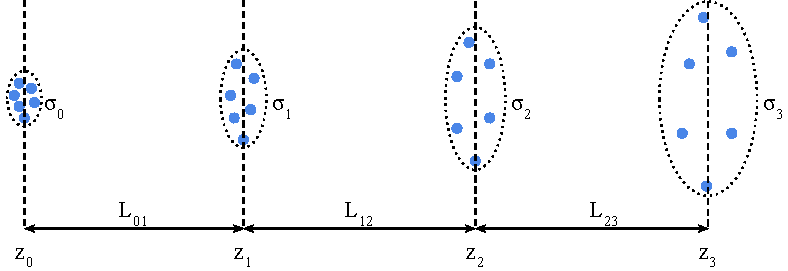
\includegraphics{part2/Figs/Multi-ProfileEmittance.pdf}
\caption{An example of a multi-profile emittance measurement conducted on an expanding beam travelling from left to right (or a shrinking beam travelling right to left).}
\label{figure:multiprofileexample}
\end{figure}

With an initial beam, $\sigma_0$, measured at $z_1, z_2$ and $z_3$ as shown in Figure~\ref{figure:multiprofileexample} then $\sigma_{11}^1$, $\sigma_{11}^2$, and $\sigma_{11}^3$ are know and we can write 
\begin{align}
\sigma_{11}^1 &= \sigma_{11}^0 +2L_{01}\sigma_{12}^0 + L_{01}^2\sigma_{22}^0 \notag\\
\sigma_{11}^2&= \sigma_{11}^0+2(L_{01}+L_{12})\sigma_{12}^0 + (L_{01}+L_{12})^2\sigma_{22}^0 \notag\\
\sigma_{11}^3&= \sigma_{11}^0+2(L_{01}+L_{12}+L_{23})\sigma_{12}^0 + (L_{01}+L_{12}+L_{23})^2\sigma_{22}^0 \label{eq:multiprofilesolution}
\end{align}

Which can easily be solved for $\sigma_0$ thus allowing the calculation of the emittance with Equation~\ref{eq:emittancewithdeterminant}.

\subsection{Quadrupole Method}

The quadrupole method is similar to the multi-profile method but requires only a single location to measure the beam width and a well characterised variable lens such as a quadrupole lens.
A quadrupole lens with a magnetic field gradient of $G$ has the transfer matrix in the focusing plane of
\begin{equation}
\mathbf{R}_f = \begin{pmatrix} \cos kl & (1/k)\sin kl\\
-k\sin kl & cos kl\end{pmatrix},
\end{equation}
where $l$ is the effective length of the quadrupole, $k^2=G/B\rho$ is the quadrupole strength and $B\rho$ is the magnetic rigidity of the particles in the assumed central trajectory.
The matrix in the defocusing palne is
\begin{equation}
\mathbf{R}_d = \begin{pmatrix} \cosh kl & (1/k) \sin kl\\
k \sinh kl & \cosh kl \end{pmatrix}
\end{equation}

A beam measured a distance $L$ away from the quadrupole will have undergone the transformation $\mathbf{R}=\mathbf{R}_L\mathbf{R}_f$ on one axis and $\mathbf{R}=\mathbf{R}_L\mathbf{R}_d$ on the other.
The symmetric beam matrix for the beam before the lens can then be determined from a series of beam profile measurements with different focusing strengths.
The main advantage of this measurement is that is only requires a single beam monitor location.

Due to the ad-hoc nature of the magnetic lenses used in the \gls{caes} this method is not practical, especially in comparison with the ease of the other methods.

\section{Simulation}

I didn't really do much simulation..... Remove this section? Or do some simulations.


\subsection{Pepperpots}

\subsection{Multiple Profile Method}

\subsection{Quadrupole Method}

\subsection{Streaking}

\subsubsection{Electron Energy}

Measurement resolution


Spot size


Stability/wrangling difficulty.


\subsubsection{Flux}

This is useful to know.
How much flux is required to get single shot measurements?
How does this match up to other charged particle sources?

\subsection{Measurement Resolution}

May be covered in other sections.


\section{Experimental Setup}

A number of modifications were made to the \gls{caeis} to prepare it for the streaked emittance measurements and there were a number of restrictions on various parameters due to the precise setup of the apparatus.
The \gls{caeis} was operated in electron mode for these measurements due to the available magnetic optics and the larger emittance expected from electrons {\color{red}(why do we expect greater emittance?)} which would reduce the likelyhood of the measurements being resolution limited.

See Chapter~\ref{chapter:setup} for a more detailed description of the \gls{caeis} and Figure~\ref{figure:emittance_schematic} for a schematic of the setup used for the measurements in this chapter.

\begin{figure}
\center
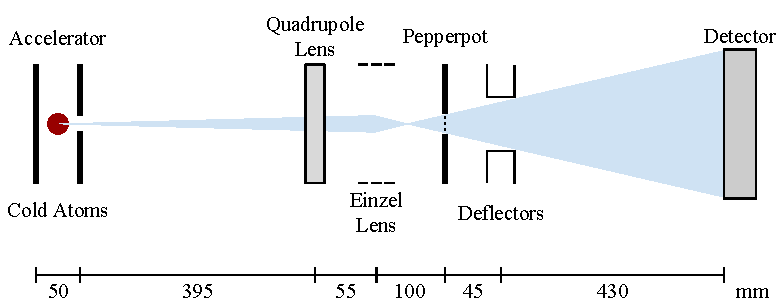
\includegraphics{part2/Figs/EmittanceApparatusSchematic.pdf}
\caption{A schematic of the experimental apparatus with relavent dimensions. The blue region indicates the electron beam envelope.}
\label{figure:emittance_schematic}
\end{figure}

\subsection{Beam Optics}
The quadrupole electron optics discussed in Section \ref{section:quadrupole} were use to reduce the astigmatism present in the electron beam as discussed in the aforementioned section. When focussing was required the Einzel lens was used.

A number of permanent magnets were used to steer the beam through the various apertures and onto the detector.
Care was taken to attempt to keep the beam on the central axis of the apparatus.


More detail (quadrupole currents, Einzel currents, focal arrangement for various tasks)

\subsection{Beam Energy}

\subsection{Bellows}

\subsection{Streaking}

\subsubsection{Deflectors}

\subsubsection{Electronics}

\subsection{Samples}

\section{Results}

\section{Conclusion}
What kind of source will this technique be useful for?
What could be learned from it?
